\section{CRUZAMENTO}
\label{sec:2cruzamento}

O operador de cruzamento (recombinação sexual) introduz diversidade na população por produzir novos indivíduos (filhos) que são compostos por partes 
retiradas de cada um dos pais. Os pais são escolhidos através dos métodos de seleção apresentados na secção \ref{sec:2selecao}.
O método mais comum de cruzamento é o cruzamento de subárvore \citep{Koza1992} que funciona da seguinte forma:

\begin{itemize}
  \item {Seleciona dois indivíduos (pais) utilizando um método de seleção}
  \item {Seleciona uma subárvore aleatória em cada um dos pais. A raíz dessa subárvore é o nó ou ponto de cruzamento\footnote{É 
  comum, e conveniente, que subárvores constituídas por símbolos terminais ou pelo nó-raiz sejam selecionadas
  com probabilidade baixa em relação as outras pois esta é provavelmente uma das causas do fenómeno conhecido por \emph{bloat},
  que é o crescimento excessivo das árvores sem uma correspondente melhoria da \emph{fitness}.}}
  \item {Cria dois novos indivíduos (filhos) por trocar as duas subárvores selecionadas entre os pais.}
\end{itemize}

A \figref{Figura261} ilustra um exemplo de um cruzamento de subárvore.

%\begin{figure}[H]
%	\centering
%	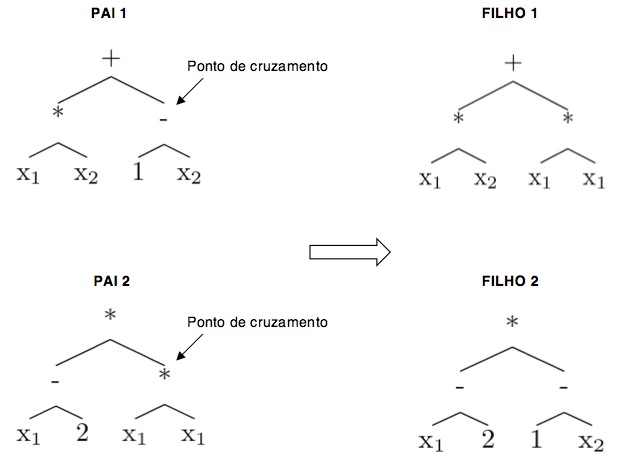
\includegraphics[width=0.75\textwidth]{figures/3}
%	\caption{Exemplo de um cruzamento de subárvore}
%	\label{Figura261}
%\end{figure}

\begin{figure}[H]
	\centering
	\begin{forest}
		for tree={child anchor=north}
		[, phantom, s sep = 2.5cm,
			%for tree={circle, draw}
			[{Pai 1}, name=pai1, baseline, for children={no edge}
				[$+$,circle,draw,
					[$*$,circle,draw
						[$x_1$,circle,draw]
						[$x_2$,circle,draw]
					]
					[,phantom]
					[$-$,name=p1p,circle,draw,fill=gray,tikz={\node [draw,red,fit to tree,dashed] {};}
						[$1$,circle,draw,name=cima]
						[$x_2$,circle,draw]
					]
				]
			]
			[{Pai 2}, name=pai2, baseline, for children={no edge}, below = 5.5cm
				[$*$,circle,draw,
					[$-$,circle,draw
						[$x_1$,circle,draw]
						[$2$,circle,draw]
					]
					[,phantom]
					[$*$,circle,draw, name=p2p,fill=gray,tikz={\node [draw,red,fit to tree,dashed] {};}
						[$x_1$,circle,draw,name=baixo]
						[$x_1$,circle,draw]
					]
				]
			]
			[{Filho 1}, name=filho1, baseline, for children={no edge}
				[$+$,circle,draw,
					[$*$,circle,draw
						[$x_1$,circle,draw]
						[$x_2$,circle,draw]
					]
					[,phantom]
					[$*$,circle,draw,name=f1p, tikz={\node [draw,red,fit to tree,dashed] {};}
						[$x_1$,circle,draw]
						[$x_1$,circle,draw]
					]
				]
			]
			[{Filho 2}, name=filho2, baseline, for children={no edge}, below = 5.5cm
				[$*$,circle,draw,
					[$-$,circle,draw
						[$x_1$,circle,draw]
						[$2$,circle,draw]
					]
					[,phantom]
					[$-$,circle,draw,name=f2p,tikz={\node [draw,red,fit to tree,dashed] {};}
						[$1$,circle,draw]
						[$x_2$,circle,draw]
					]
				]
			]	
		]
		\draw[arrows={-triangle 45},dashed,color=red] (p1p) to [out=south east,in=north east] (f2p);
		\draw[arrows={-triangle 45},dashed,color=red] (p2p) to [out=north east,in=south west] (f1p);
	\end{forest}
	\caption{Exemplo de cruzamento de subárvore. O nó cinzento é o ponto de cruzamento}
	\label{Figura261}
\end{figure}



